\section{Technologien}

\subsection{Software-Defined Access (SDA)}
Cisco bietet mit SDA eine automatisierte End-to-End-Segmentierung um den Benutzer-, Geräte- und Anwendungsverkehr zu trennen, ohne das Netzwerk neu zu gestalten. Durch diesen automatisierten Benutzerzugriff ermöglicht SDA Einrichtungen innert kürzester Zeit. Durch diese enorme Vereinfachung wird eine zusätzliche Sicherheit und Skalierung des Betriebs gewonnen. Ebenso wird die Transparenz deutlich erhöht und die schnelle Bereitstellung neuer Dienste gewährleistet. Durch die Automatisierung von täglichen Aufgaben wie Konfiguration, Bereitstellung und Troubleshooting reduziert SDA die Zeit für Netzwerkanpassungen, verbessert die Problemlösungszeit und reduziert die Auswirkungen von Sicherheitsverletzungen.\\
\\
So können Organisationen sicherstellen, dass für jeden Benutzer oder jedes Gerät mit jeder Anwendung die richtigen Richtlinien festgelegt werden über das Netzwerk. Dies wird mit einer einzigen Netzwerkstruktur über LAN und WLAN erreicht, wodurch ein konsistente Benutzererfahrung überall ohne Kompromisse bei der Sicherheit. \\
\\
SDA wird aus mehreren Komponenten zusammengesetzt. Dazu gehört das DNA Center, welches die grundsätzliche Funktion des Netzwerks sicherstellt, sowie eine ISE, welches die Benutzeridentitäten und Profile verwaltet. \cite{sda-definition}

\subsubsection{Campus Fabric} \label{CampusFabric}
Um eine konsistente Benutzererfahrung zu erreichen, braucht man eine Switching-Infrastruktur mit der sich der Zugang zu bestimmten IP-Subnetzen ortsunabhängig realisieren lässt. \cite{campusfabric-introduction} \\

\begin{figure}[H]
	\centering
	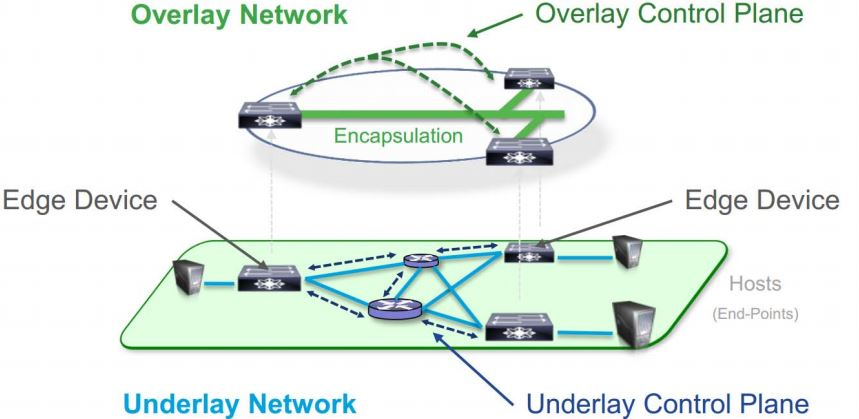
\includegraphics[height=6cm]{img/campusfabric.jpg}
	\caption{Aufteilung des Campus Fabric in Underlay und Overlay Netzwerk \cite{sda-1-0-whitepaper}}
	\label{fig:Campus Fabric}
\end{figure}

Die SDA Architektur wird durch die für den Campus implementierte Fabric Technologie unterstützt, welche die Verwendung virtueller Netzwerke (Overlay Network) in einem physischen Netzwerk (Underlay Network) ermöglicht, um alternative Topologien für die Verbindung von Geräten zu erstellen. Overlay Netzwerke werden in Data Center häufig verwendet, um die Mobilität von virtuellen Maschinen über Layer 2 und Layer 3 bereitzustellen. Dies wird beispielsweise mit Application Centric Infrastructure (ACI), VXLAN und Fabric Path realisiert. Overlay Netzwerke werden auch in Wide Area Netzwerken (WAN) verwendet, um sicheres Tunneling von Remote-Standorten aus zu ermöglichen. Beispiele dafür sind die Protokolle Multiprotocol Label Switching (MPLS), Dynamic Multipoint VPN (DMVPN) und Generic Routing Encapsulation (GRE). \cite{sda-designguide}

\paragraph{Overlay Network}
Die Fabric bildet ein Overlay Netz. Das Overlay Netz bildet eine virtuelle Topologie um Geräte miteinander zu verbinden, welches auf einer beliebigen physischen Underlay Topologie aufgebaut ist. Das Overlay Netzwerk verwendet oft alternative Weiterleitungsattribute, um zusätzliche Dienste bereitzustellen, die nicht vom Underlay Netzwerk bereitgestellt werden. 
Der Data Plane Traffic und die Control Plane Signalisierung sind in jedem virtualisierten Netzwerk enthalten, wobei zusätzlich zu der Isolation von dem Underlay Netzwerk eine Isolation zwischen den Netzwerken aufrechterhalten wird. Die SDA Fabric implementiert die Virtualisierung, indem sie den Benutzerdatenverkehr über IP-Pakete einkapselt, die an den Grenzen des Fabrics bereitgestellt und abgeschlossen werden.
Overlay Netzwerke können über alle oder eine Teilmenge der Underlay Netzwerkgeräte hinweg ausgeführt werden. Mehrere Overlay Netzwerke können aber auch über das gleiche Underlay Netzwerk laufen, um Multi-Tenancy durch Virtualisierung zu unterstützen. Die Netzwerkvirtualisierung, welche sich ausserhalb der Fabric erstreckt, wird mithilfe herkömmlicher Virtualisierungstechnologien wie Virtual Routing and Forwarding (VRF)-Lite und MPLS VPN beibehalten.
Der IPv4 Multicast wird gekapselt und an interessierte Fabric Edge Switches gesendet, welche den Multicast wiederum entkapseln und an die Empfänger weiterleiten. Ist der Empfänger ein drahtloser Client, so wird der Multicast (genau wie ein Unicast) durch den Fabric Edge in Richtung des Access Point (AP) mit dem Multicast-Empfänger gekapselt. Die Multicast Quelle kann entweder innerhalb oder ausserhalb eines Overlay Netzwerkes vorhanden sein. \cite{sda-designguide}

\paragraph{Underlay Network}
Das Underlay Netzwerk wird durch die physischen Switches und Router definiert, die Teil des SDA Netzwerks sind. Jegliche Geräte die dem Underlay Netzwerk angehören, müssen über ein Routing Protokoll eine IP Konnektivität herstellen. Obwohl auf dem Underlay beliebige Topologie- und Routing-Protokolle verwendet werden können, wird von Cisco die Implementierung einer gut überlegten Layer 3 Grundlage bis zum Campus Edge empfohlen, um die hohe Leistung, sowie Skalierbarkeit und Verfügbarkeit des Netzwerkes zu gewährleisten. 
Um dieses Ziel für die Underlay Deployments zu erreichen, welche nicht manuell erstellt werden, werden bei der DNA Center LAN-Automatisierung neue Netzwerke mit einem Intermediate System to Intermediate System (IS-IS)-Routing Access Design bereitgestellt. Obwohl es viele Alternativen gibt, bietet diese Auswahl betriebliche Vorteile wie zum Beispiel dem Nachbarschaftsaufbau ohne IP-Protokollabhängigkeiten, Peering-Fähigkeit unter Verwendung von Loopback-Adressen und agnostische Behandlung von IPv4-, IPv6- und Nicht-IP-Verkehr. \cite{sda-designguide}

\paragraph{Fabric Data Plane and Control Plane}
SDA konfiguriert das Overlay Netzwerk mit einer Fabric Data Plane mithilfe der VXLAN Technologie. VXLAN kapselt und durchtunnelt komplette Layer 2 Frames über das Underlay Netzwerk, wobei jedes Overlay Netzwerk durch eine Virtual Extensible LAN Network Identifier (VNI) identifiziert wird. Der VXLAN Header enthält auch die Security Group Tags (SGTs), die für die Mikrosegmentierung erforderlich sind.

Das Mapping und Auflösen von Endpunkten, die VXLAN-Tunnelendpunkten (VTEPs) zugeordnet sind, erfordert ein Control Plane Protokoll, und SD Access verwendet LISP für diese Aufgabe. LISP bietet den Vorteil, dass das Routing nicht nur auf der IP-Adresse als Endpunktkennung (EID) für ein Gerät basiert, sondern auch eine zusätzliche IP-Adresse als Routing Locator (RLOC) zur Verfügung stellt, um den Netzwerkstandort dieses Geräts darzustellen. Die EID- und RLOC-Kombination bietet alle erforderlichen Informationen für die Weiterleitung von Datenverkehr, selbst wenn ein Endpunkt eine unveränderte IP-Adresse verwendet, wenn er an einem anderen Netzwerkstandort angezeigt wird. Gleichzeitig ermöglicht die Entkopplung der Endpunktidentität von ihrem Standort, dass Adressen in demselben IP-Teilnetzwerk hinter mehreren Layer 3 Gateways verfügbar sind, gegenüber der Eins-zu-eins-Kopplung von IP-Teilnetzwerk mit Netzwerk Gateway in herkömmlichen Netzwerken Beispiel für zwei Subnetze, die Teil des Overlay Netzwerks sind. Die Subnetze erstrecken sich über physisch getrennte Layer 3 Geräte. Die RLOC-Schnittstelle ist die einzige routbare Adresse, die zum Herstellen der Verbindung zwischen Endpunkten desselben oder eines anderen Subnetzes erforderlich ist. Weitere detailliertere Informationen zu LISP und VXLAN folgen in den nächsten Kapiteln. \cite{sda-designguide} \\


In der nachfolgenden Abbildung ist der Aufbau eines Campus Fabric mit allen Komponenten etwas detaillierter aufgezeigt.

\begin{figure}[H]
	\centering
	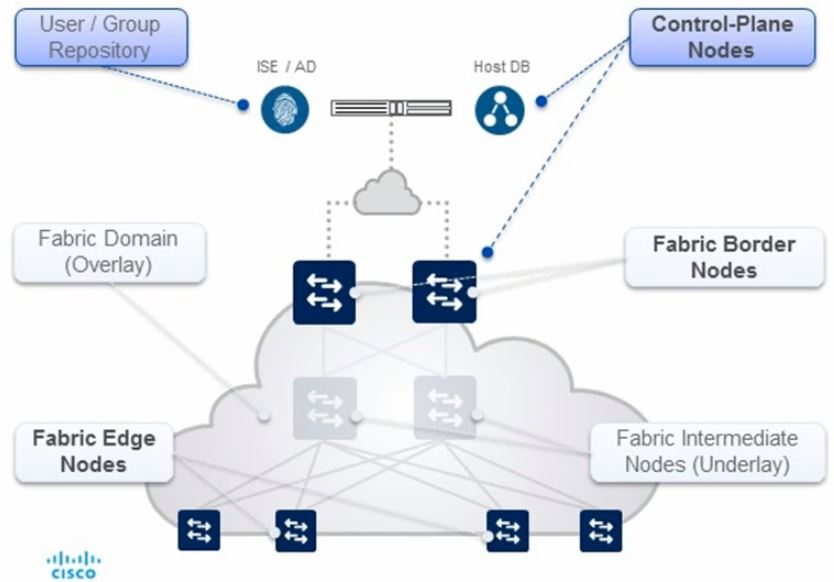
\includegraphics[height=8cm]{img/fabric-roles&terminology.jpg}
	\caption{Fabric Rollen und Terminologie \cite{webinar-sda-troubleshooting}}
	\label{fig:Fabric Rollen und Terminologie}
\end{figure}

Dieses Campus Fabric besteht aus folgenden Elementen:
\begin{itemize}	
	\item User/Group Repository: Ein externes ID-Speichergerät (z. B. ISE oder AD) kann verwendet werden, um eine dynamische Zuordnung von Benutzer/Gerät zu Gruppen bereitzustellen
	\item Control-Plane-Nodes: Ein Map System, das die Beziehung eines Endpoints zu einem Gateway (Edge oder Border) verwaltet
	\item Border-Nodes: Das L3-Gateway-Gerät (Core), das externe L3-Netzwerke mit dem Fabric verbindet
	\item Edge-Nodes: Das L3-Gateway-Gerät (Access oder Distribution), das Endpoints mit Fabric verbindet
	\item Intermediate Nodes: Normale L3 (IP) Forwarder im Underlay Netzwerk
\end{itemize}

\paragraph{Control-Plane Nodes}
Der SDA Fabric Control Plane basiert auf der LISP Map Server (MS) und LISP Map Resolver (MR), welche auf demselben Node kombiniert sind. Die Funktion des Control Planes wird am Border Node oder Dedicated Node instanziiert. Der Control Plane Node ermöglicht folgende Funktionen: \cite{sda-designguide}
\begin{itemize}	
	\item Host Tracking Database: Die Host Tracking Database (HTDB) ist ein zentrales Repository von EID zu Fabric Edge Nodes Verbindungen.
	\item Map Server: Der LISP-MS wird verwendet, um die HTDB mit Registrierungsnachrichten von Fabric-Edge-Geräten zu füllen.
	\item Map Resolver: Der LISP MR wird verwendet, um auf Map Abfragen von Fabric-Edge-Geräten zu reagieren, die RLOC-Mapping-Informationen für Ziel-EIDs anfordern.
\end{itemize}

\paragraph{Fabric Border Nodes}
Die Fabric Border Nodes dienen als Gateway zwischen der SDA Fabric Domäne und dem Netzwerk ausserhalb der Fabric. Der Fabric Border Node ist für die Netzwerkvirtualisierung und die SGT Propagierung vom Fabric zum Rest des Netzwerks verantwortlich. Die Fabric Border Nodes können entweder als Gateway für bestimmte Netzwerkadressen, z.B. ein Netzwerk für gemeinsam genutzte Dienste, oder in einer Standard-Border-Rolle, die für das Internet oder einen gemeinsamen Austrittspunkt aus einer Fabric nützlich ist. Border Nodes implementieren die folgenden Funktionen: \cite{sda-designguide}
\begin{itemize}	
	\item Advertisement von EID Subnetzen: SDA konfiguriert das Border Gateway Protocol (BGP) als bevorzugtes Routing-Protokoll zum Anbieten der EID-Präfixe ausserhalb der Fabric und der für EID-Subnetze von ausserhalb der Fabric bestimmte Verkehr durchläuft die Border Nodes. Diese EID-Präfixe werden nur in den Routingtabellen am Border angezeigt. Im gesamten Fabric werden die EID-Informationen über den Fabric Control Plane abgerufen.
	\item Fabric Domain Exit Point: Der Standard Fabric Border ist der Gateway für den letzten Exit Point für die Fabric Edge Nodes. Dies wird mithilfe der LISP Proxy Tunnel Funktionalität implementiert.
	\item Mapping von LISP Instanzen zu VRF: Der Fabric Border kann die Netzwerkvirtualisierung von innerhalb des Fabrics nach ausserhalb des Fabrics erweitern, indem externe VRF Instanzen verwendet werden, um die Virtualisierung beizubehalten.
	\item Policy Mapping: Der Fabric Border Node bildet auch SGT-Informationen aus dem Fabric ab, die beim Verlassen des Fabric entsprechend gepflegt werden. Tags aus dem VXLAN-Header werden Cisco Meta Data (CMD) zugeordnet, wenn Inline-Tagging-Funktionen verwendet werden, oder alternativ werden die Tags über das SGT-Austauschprotokoll (SXP) transportiert, sodass eine nahtlose Integration in die Cisco TrustSec-Lösung möglich ist.
\end{itemize}


\paragraph{Fabric Edge Nodes}
Die SDA Fabric Edge Nodes entsprechen einem Access Layer Switch in einem herkömmlichen Campus-Design. die Edge Nodes implementieren ein Layer 3 Access Design mit den folgenden Fabric Funtkionen: \cite{sda-designguide}
\begin{itemize}	
	\item Endpunktregistrierung: Nachdem ein Endpunkt von der Fabric Edge erkannt wurde, wird er einem lokalen Host-Tracking Datenbank (EID Tabelle) hinzugefügt. Das Edge Gerät gibt auch eine LISP Map Register Nachricht aus, um den Control Plane Node über den erkannten Endpunkt zu informieren, damit dieser die Informationen in die HTDB einfügen kann.
	\item Zuordnung von Benutzer zu virtuellem Netzwerk: Endpunkte werden in virtuellen Netzwerken platziert, indem der Endpunkt einem VLAN zugewiesen wird, das einer LISP-Instanz zugeordnet ist. Die Zuordnung von Endpunkten zu VLANs kann statisch oder dynamisch mit 802.1X erfolgen. Eine SGT wird ebenfalls zugewiesen, und eine SGT kann verwendet werden, um Segmentierung und Richtliniendurchsetzung an der Fabric Edge bereitzustellen.
	\item Anycast Layer 3 Gateway: Ein gemeinsamer Gateway (IP- und MAC-Adressen) kann an jedem Knoten verwendet werden, der sich ein gemeinsames EID-Subnetz teilt, um eine optimale Weiterleitung und Mobilität zwischen verschiedenen RLOCs zu gewährleisten.
	\item LISP Forwarding und VXLAN Encapsulation/De-Encapsulation: Anstelle einer typischen routingbasierten Entscheidung fragen die Fabric Edge Nodes den Map Server an, um den der Ziel-IP zugeordneten RLOC zu ermitteln und den Verkehr mit VXLAN-Headern zu kapseln. Schlägt die Abfrage fehl, so wird der Traffic an einen Default Fabric Border gesendet, auf dem die globale Routing-Tabelle für das Weiterleiten verwendet wird. Die von Map Server empfangene Antwort wird im LISP Map Cache gespeichert. 
\end{itemize} 

\paragraph{Fabric Intermediate Nodes (Underlay)}
Die Fabric Intermediate Nodes sind Teil des Layer 3 Netzwerk, das für Verbindungen zwischen den Edge Nodes zu den Border Nodes verwendet wird. Im Falle das ein 3 Tier Campus Design mit einem Core, Distribution und Access Layer verwendet wird, sind die  Intermediate Nodes äquivalent zu Distribution Switches. Intermediate Nodes routen nur den IP-Verkehr innerhalb der Fabric. \cite{sda-designguide}

\subsubsection{Architektur}
Cisco SDA kann grob in fünf Layer aufgeteilt werden.
\begin{figure}[H]
	\centering
	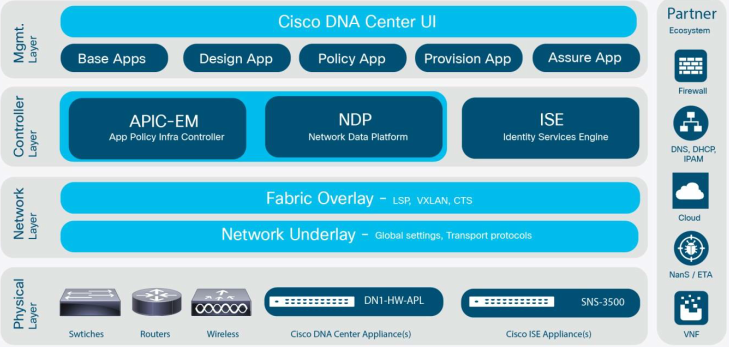
\includegraphics[width=1\linewidth]{img/cisco-sda-architecture.png}\\[1px]
	\caption{SDA Architektur}
	\label{fig:SDA Architektur}
\end{figure}


\subsection{Cisco Digital Network Architecture Center (Cisco DNA-Center)}
Im Zentrum der Automatisierung der SDA Lösung steht das Cisco DNA Center. DNA Center ist ein Controller für die Planung und Vorbereitung, Installation und Integration. SDA ist eines der vielen Softwarepakete, die auf dem DNA Center laufen und ist die Grundlage des Cisco DNA. Es ermöglicht den Netzwerkzugriff in Minuten für jeden Benutzer oder jedes Gerät für jede Anwendung, ohne Kompromisse. Bei SDA folgen die festgelegten Richtlinien automatisch dem Benutzer über alle Netzwerkdomänen hinweg.
DNA Center ist das zentrale Überwachungs-Dashboard für Netzwerke, mit dem alle Cisco DNA-Produkte und -Lösungen verwaltet werden können.

DNA Center gibt die Möglichkeit unter einem Grafischen Nutzer Interface direkt mit APIC(Application Policy Infrastructure Controller)-EM 2.x Applikationen mit der Identity Services Engine (ISE) und mit Network Data Plattform (NDP) unserer Assurance und Analytics Plattform zu sprechen. Alle Parameter die angezeigt oder konfiguriert werden müssen, kann man unter DNA Center ausführen und muss nicht zwischen den einzelnen Modulen und Oberflächen hin und her springen.
\begin{figure}[H]
	\centering
	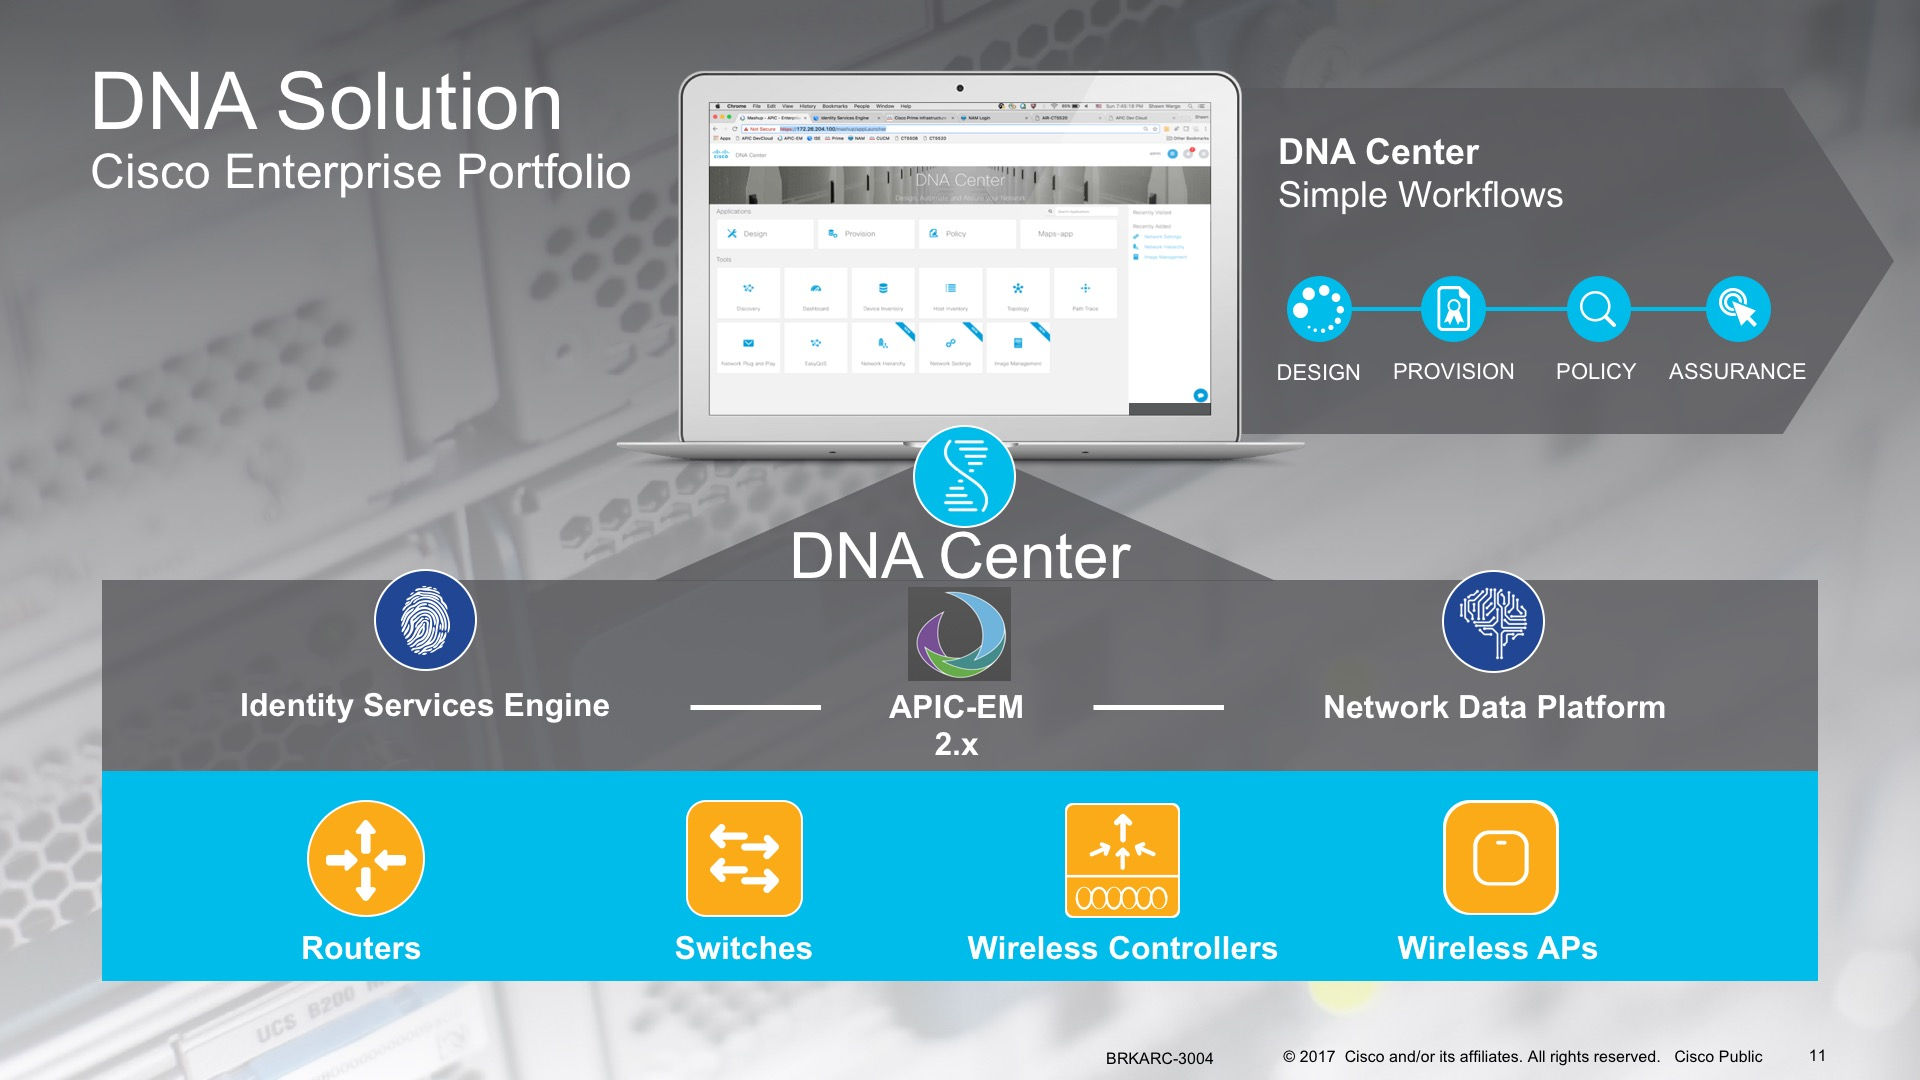
\includegraphics[height=7cm]{img/DNAC-1.jpg}
	\caption{DNA Solution}
	\label{fig:Aufbau einer DNA Solution}
\end{figure}
APIC-EM 2.x automatisiert dann die notwendigen Konfigurationen und spricht mit dem Netzwerk. Auch die Integration von IP Address Management Lösungen wie z.B. Infoblox werden nur über die DNA Center Oberfläche konfiguriert. Dies geschieht über verschiedene API-basierte Datenaustauschmechanismen sowie einen automatisierten Zertifikataustausch für Partnersysteme (zum Beispiel Cisco ISE). \cite{sda-whitepaper} \\

\begin{figure}[H]
	\centering
	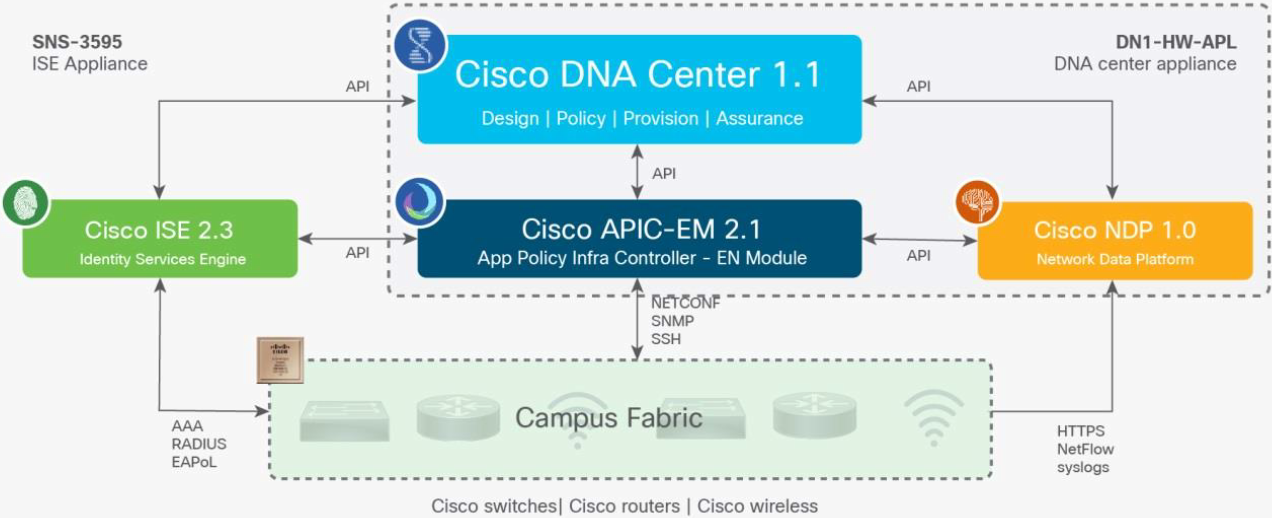
\includegraphics[width=1\linewidth]{img/ControllerLayer.png}\\[1px]
	\caption{SDA Architektur} 
	\label{fig:SDA Architektur}
\end{figure}

Das DNA Center verwaltet zentral folgende vier Hauptbereiche: \cite{sda-designguide}

\begin{figure}[H]
	\centering
	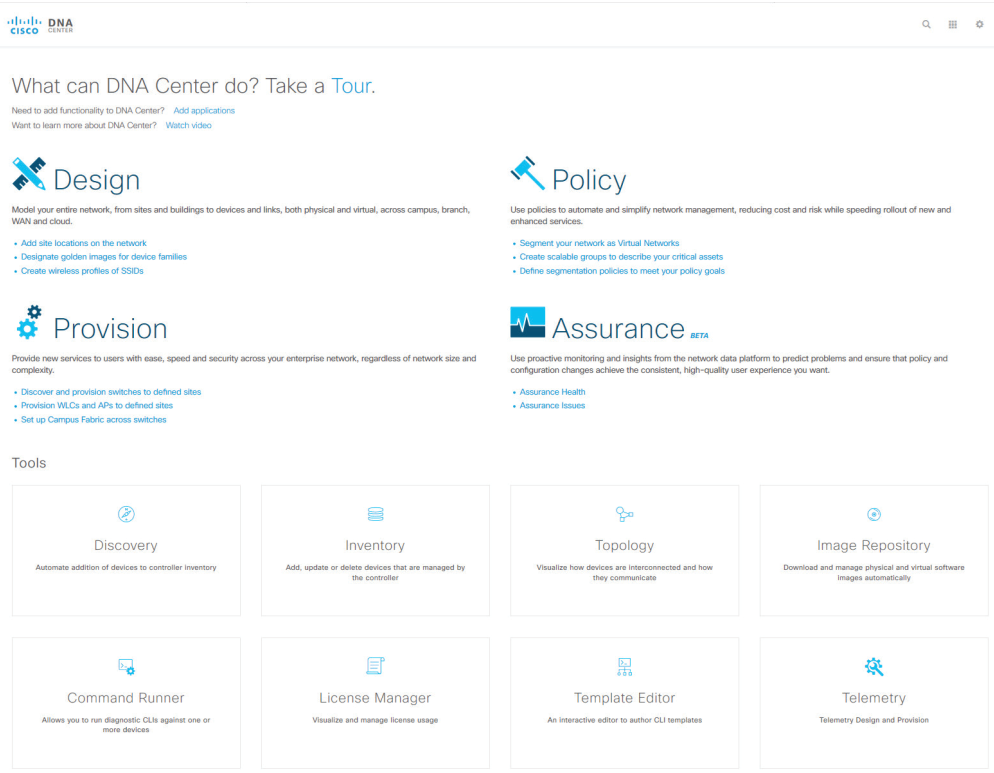
\includegraphics[height=10cm]{img/DNA-Dashboard.png}
	\caption{DNA Dashboard}
	\label{fig:DNA Dashboard}
\end{figure}


\paragraph{Design}
Konfiguriert globale Geräteeinstellungen, Netzwerkstandortprofile für die physische Geräteinventur, DNS, DHCP, IP-Adressierung, Software-Image-Verwaltung, Plug-and-Play und Benutzerzugriff.
\paragraph{Policy}
Definiert die Geschäftsabsicht für die Bereitstellung im Netzwerk, einschließlich der Erstellung virtueller Netzwerke, der Zuweisung von Endpunkten zu virtuellen Netzwerken und der Definition von Richtlinienverträgen für Gruppen.
\paragraph{Provision}
Stellt Geräte für das Management bereit und erstellt Fabric-Domänen, Control Plane Nodes, Border Nodes, Edge Nodes, Fabric-Wireless und externe Konnektivität.

\paragraph{Assurance}
Aktiviert das Health-Score-Dashboard, Client/Gerät-360 Grad-Ansichten, Knoten-, Client- und Pfad-Traces. DNA Center unterstützt die Integration mithilfe von APIs. Zum Beispiel ist die Integration von IP-Adressen von Infoblox und die Integration von Policy Enforcement mit ISE über DNA Center verfügbar. Ein umfassendes Set von Northbound-REST-APIs ermöglicht Automatisierung, Integration und Innovation.



\subsection{Identity Service Engine (ISE)}
Cisco ISE ist ein wesentlicher Bestandteil von SDA für die Richtlinienimplementierung. Mit der Cisco ISE können Benutzer und Geräte, die mit dem Unternehmensnetzwerk verbunden sind, angezeigt und gesteuert werden. Das alles von einer zentralen Stelle aus. ISE ermöglicht es einem Netzwerkadministrator, Zugriffsrichtlinien für kabelgebundene und drahtlose Endpunkte basierend auf Informationen zentral zu steuern, die über RADIUS-Nachrichten gesammelt werden, die zwischen dem Gerät und dem ISE-Knoten übertragen werden. Dies wird auch als Profiling bezeichnet. Die Profiling-Datenbank wird regelmäßig aktualisiert, um mit den neuesten und besten Geräten Schritt zu halten, so dass keine Lücken in der Gerätesichtbarkeit bestehen. \\
\\
Im Wesentlichen hängt ISE eine Identität an ein Gerät an, basierend auf Benutzer-, Funktions- oder anderen Attributen, um Richtliniendurchsetzung und Sicherheitskonformität bereitzustellen, bevor das Gerät autorisiert wird, auf das Netzwerk zuzugreifen. Basierend auf den Ergebnissen einer Vielzahl von Variablen kann ein Endpunkt mit bestimmten Zugriffsregeln auf das Netzwerk zugelassen werden, die auf die Schnittstelle angewendet werden, mit der er verbunden ist. Andernfalls kann er vollständig verweigert oder basierend auf den spezifischen Unternehmensrichtlinien gewährt werden. \\
\\
DNA Center bietet einen Mechanismus zum Erstellen einer vertrauenswürdigen Kommunikationsverbindung mit Cisco ISE und ermöglicht den beiden Anwendungen, Daten auf sichere Weise miteinander zu teilen. ISE integriert sich in DNA Center mit Hilfe von Cisco Platform Exchange Grid (pxGrid) und REST APIs zum Austausch von Client-Informationen und zur Automatisierung von Fabric-bezogenen Konfigurationen auf ISE. Sobald die ISE beim DNA Center registriert ist, wird jedes Gerät, das ISE entdeckt, zusammen mit der entsprechenden Konfiguration und anderen Daten an das DNA Center weitergeleitet. Benutzer können beide Anwendungen verwenden, um Geräte zu erkennen und dann sowohl DNA Center- als auch ISE-Funktionen auf sie anzuwenden, da diese Geräte in beiden Anwendungen verfügbar sind. DNA Center- und ISE-Geräte werden alle durch ihre Gerätenamen eindeutig identifiziert. \\
\\
In ähnlicher Weise werden DNA-Center-Geräte sobald sie bereitgestellt werden und zu einer bestimmten Seite in der DNA Center-Standorthierarchie gehören, an ISE übergeben. Alle Aktualisierungen an einem DNA Center-Gerät (z. B. Änderungen an der IP-Adresse, SNMP- oder CLI-Anmeldeinformationen, gemeinsamer ISE-Schlüssel usw.) werden automatisch an die entsprechende Geräteinstanz auf der ISE weitergeleitet. Wenn ein DNA Center-Gerät gelöscht wird, wird es ebenfalls aus der ISE entfernt.

\subsection{Locator ID Separation Protocol (LISP)} 
LISP ist das Produkt einer Arbeitsgruppe in der Internet Engineering Taskforce (IETF), um was wachsende Problem des doppelten Verwendungszwecks der IP-Adressen zu bereinigen. Zur Zeit wird die IP-Adresse benutzt um die Identität eines Hosts festzulegen und auch den Ort zu bestimmen, an dem er sich im Internet befindet. Dies hat zur Folge das sich bei einem Aufenthalsortwechsel auch die IP-Adresse des Hosts ändert, was bedeutet das die Identität verloren geht und die alten IP-Verbindungen verfallen. \\

\begin{figure}[H]
	\centering
	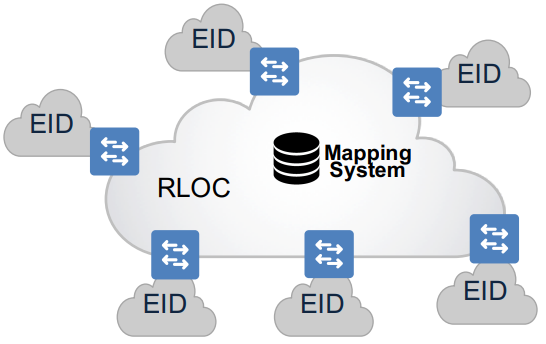
\includegraphics[height=3.5cm]{img/lisp.png}
	\caption{LISP Aufbau}
	\label{fig:LISP Aufbau}
\end{figure}

Dies soll nun durch LISP geändert werden, in dem es die Identität eines Gerätes, auch Endpoint Identifier (EID) genannt, von seinem Aufenthaltsort, auch Routing Locator (RLOC) genannt, in zwei separate Adressräume unterteilt. Das bedeutet, dass die Router in einer LISP-Architektur nur Routing-Informationen von RLOCs speichern müssen. Um Pfadinformationen eines Hosts abzurufen, kann der Router diese beim LISP-Mapping-Server abfragen, was analog wie das DNS-Mapping funktioniert. \\

LISP verwendet für SDA/Fabric eine VXLAN-Kapselung. Um die VXLAN-Kapselung für LISP zu aktivieren, muss auf dem Router der LISP Konfigurationsmodus, den Befehl für die VXLAN-Enkapsulierung verwendet werden. Dieser Befehl muss auf allen LISP-Edge-Geräten im Enterprise-Fabric konfiguriert werden: Ingress Tunnel Router (ITR), Egress Tunnel Router (ETR), Proxy Ingress Tunnel Router (PITR), Proxy Egress Tunnel Router (PETR). Wenn dieser Befehl nicht auf einem der LISP-Edge-Geräte konfiguriert wird, führt dies zu einem Verlust der Kontrolle und des Datenverkehrs.  \cite{rfc-6830}

\begin{table}[H]
	\rowcolors{2}{gray!25}{white}
	\centering
	\begin{tabularx}{\textwidth}{p{6.6cm} | X}
		\rowcolor{gray!50}
		\textbf{LISP Device} & \textbf{Function} \\
		\hline	
		ALT (Alternative Logical Topology) & Collects EID data from Map Servers (MS) and advertise aggregate EID prefix. In a deployment of multiple Map Servers, it keeps all synchronized. \\
		
		ETR (Egress Tunnel Router) and PETR (Proxy ETR) & Connects a LISP capable core network. Registers EID prefices with Map Server (MS). Decapsulates LISP packets, received from LISP core. Responds to Map-request messages with a Map-Reply by giving appropriate EID prefix. Typically, this is a CPE (customer premise equipment) router. PETR works on behalf on non-LISP domain and provides LISP-non-LISP connectivity. \\ 
		
		ITR (Ingress Tunnel Router) and PITR (Proxy Ingress Tunnel Router) & Responsible for forwarding local traffic to external destinations. Resolves RLOC for a given destination by sending Map-request to Map Resolver. Encapsulates (vxlan) traffic with LISP header. Typically, this is a Access Layer Switch. PITR works on behalf on non-LISP domain and provides LISP-non-LISP connectivity. \\
		
		XTR (X Tunnel Router) & When both ITR and ETR functions are handled by one router, it is called XTR. This is typical in practice. \\
		
		MR (Map Resolver) & Responds to Map-requests from ITR. Map-requests will be replied with a Negative Map-Reply or forwarded to appropriate ETR or ALT. \\
		
		MS (Map Server) & Registers EID space upon receiving Map-register messages from ETR. Updates ALT and MR with EID and RLOC data. \\
		
		MSMR (Map Server Map Reloader) & When a device acts as both Map Server and Map Resolver, it is called MSMR. This is typical in practice. \\
		
		EID (Endpoint ID) & Endpoint Identifier. IP addresses hidden from core network routing table. RLOC acts next-hop to reach EID space. \\
		
		RLOC (Routing Locator) & Routing Locator. Exists in global routing tables. Authoritative to reach EID space. \\
		
	\end{tabularx}
	\caption{LISP Elements}
	\label{tab:LISP Elements}
\end{table}

\subsubsection{Campus Fabric und LISP}
Im Einzug mit dem Campus Fabric wurden für bestehende LISP Namenskonzepte neue Begriffsdefinitionen zugewiesen:
\begin{itemize}
	\item "Control-Plane Node" $\approx$ "LISP Map-Server"
	\item "Edge Node" $\approx$ "LISP Tunner Router" (xTR)
	\item "Border Node" $\approx$ "LISP Proxy Tunnel Router" (PxTR)
	\item "Intermediate Node" $\approx$ "Non-LISP IP Forwarder"
\end{itemize}

\paragraph{Fabric Control-Plane Node} basiert auf einem LISP Map Server / Resolver. Führt die LISP-Host-Tracking-Datenbank aus, um Overlay-Erreichbarkeitsinformationen bereitzustellen. 
\begin{itemize}
	\item Eine einfache Host-Datenbank, die die Endpunkt-ID zu Edge-Knoten-Bindungen zusammen mit anderen Attributen verfolgt
	\item Host-Datenbank unterstützt mehrere Endpoint-ID-Lookup-Schlüssel (IPv4 / 32, IPv6 / 128 oder MAC)
	\item Empfängt Präfix-Registrierungen von Edge Nodes mit lokalen Endpunkten
	\item Beheben von Suchanforderungen von Remote-Edge-Knoten, um lokale Endpunkte zu finden
\end{itemize}

\paragraph{Fabric Edge Node} basiert auf einem LISP Tunnel Router (xTR). Bietet Konnektivität für Benutzer und Geräte, die mit dem Fabric verbunden sind.
\begin{itemize}
	\item Verantwortlich für das Identifizieren und Authentifizieren von Endpunkten
	\item Registrieren von Endpunkt-ID mit dem Control-Plane Node(s)
	\item Bietet Anycast L3 Gateway für verbundene Endpunkte
	\item Host-Datenverkehr von und zu Endpunkten, die mit dem Fabric verbunden sind, verkapseln/entkapseln
\end{itemize}

\paragraph{Fabric Border Node} basiert auf einem LISP Proxy Tunnel Router (PxTR). Der gesamte Verkehr, der das Fabric betritt oder verlässt, durchläuft diesen Knotentyp.
\begin{itemize}
	\item Verbindet traditionelle L3-Netzwerke und / oder verschiedene Fabric-Domänen mit der lokalen Domäne
	\item Wo zwei Domains Endpoint Erreichbarkeit und Richtlinieninformationen austauschen
	\item Verantwortlich für die Übersetzung von Kontexten (VRF und SGT) von einer Domäne in eine andere
	\item Stellt einen Domänenexitpunkt für alle Edge-Knoten bereit
\end{itemize}

\subsection{Virtual Extensible LAN (VXLAN)}
VXLAN ist ein Encapsulation-Protokoll, um ein Overlay-Netzwerk auf einer existierenden Layer 3 Infrasturktur laufen zu lassen. VXLAN wurde ursprünglich von Cisco Systems, VMware und Arista Network entwickelt und ist einer der IETF festgelegten Standards (RFC 7348). \cite{rfc-7348} \\
\\
Technisch gesehen erzeugt ein VXLAN logische Layer 2 Netzwerke, die dann in standardmässige Layer 3 Pakete eingepackt werden. VXLAN dient dazu um in sehr grossen Netzwerkumgebung die Probleme zu lösen, die durch beschränkte Anzahl von VLANS betroffen sind. Mit VXLAN sind insgesamt 16’777’215 (24 Bit) Layer 2 Umgebungen möglich, die ihrerseits wieder jeweils 4096 VLANs beinhalten können. 

\subsubsection{VXLAN Encapsulation}
Die Data Plane basiert auf VXLAN, im Gegensatz zur Control Plane, welche auf LISP basiert. Die VXLAN-Kapselung ist IP/UDP-basiert, was bedeutet, dass sie von jedem IP-basierten Netzwerk (Legacy- oder nicht-Cisco-Netzwerk) weitergeleitet werden kann und effektiv den Overlay-Aspekt des SD-Access-Fabric erzeugt. Die VXLAN-Kapselung wird (statt der LISP-Kapselung) aus zwei Hauptgründen verwendet. VXLAN umfasst den Source Layer 2 (Ethernet) -Header (LISP nicht) und bietet auch spezielle Felder für zusätzliche Informationen, wie die ID des virtuellen Netzwerks (VN) und die ID der Gruppe (Segment). \cite{sda-whitepaper}\\

Diese Technologie bietet mehrere Vorteile für SD-Access, z. B. Unterstützung für virtuelle Layer 2 und Layer 3 Topologien (Overlays) und die Möglichkeit, über jedes IP-basierte Netzwerk mit integrierter Netzwerksegmentierung (VRF/VN) und gruppenbasierter Richtlinie zu arbeiten. \\ 

In SD-Access wurden einige Verbesserungen der ursprünglichen VXLAN-Spezifikationen hinzugefügt, insbesondere die Verwendung von Sicherheitsgruppen-Tags (SGTs). Dieses neue VXLAN-Format ist derzeit ein IETF-Entwurf, der als Gruppenrichtlinienoption (oder VXLAN-GPO) bekannt ist.

\begin{figure}[H]
	\centering
	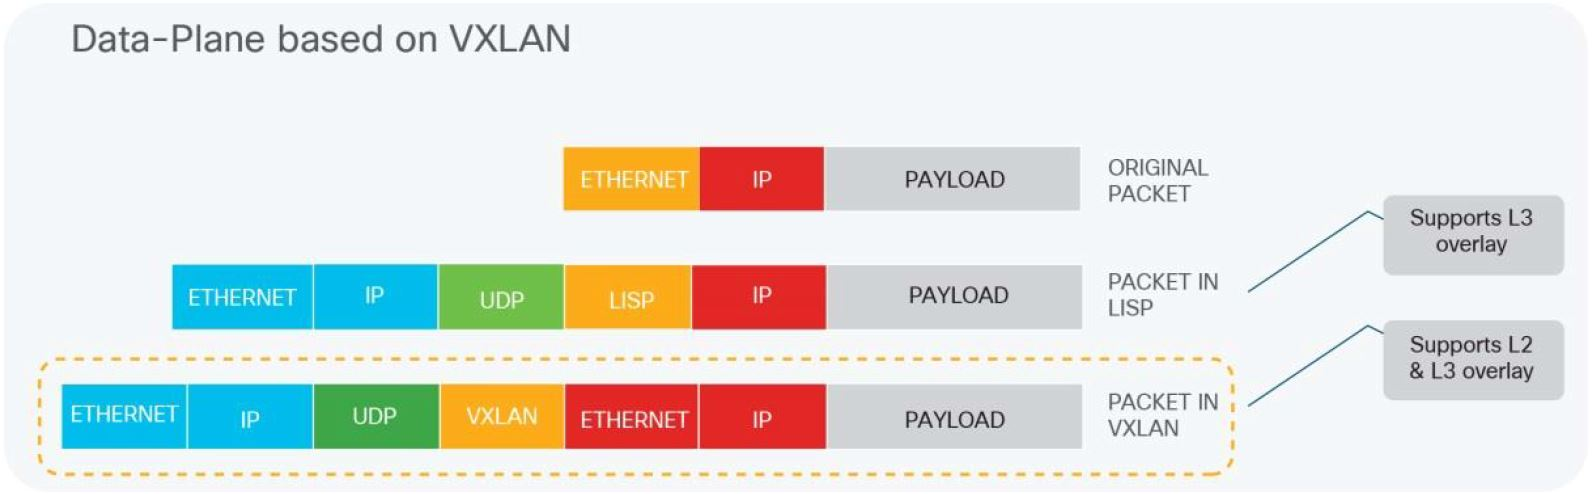
\includegraphics[height=4.5cm]{img/vxlan-encapsulation.jpg}
	\caption{VXLAN Encapsulation}
	\label{fig:VXLAN Encapsulation}
\end{figure}

Die Fabric Data-Plane bietet folgendes:
\begin{itemize}
	\item Underlay Adressanzeige und -zuordnung
	\item Automatischer Tunnelaufbau (Virtuelle Tunnelendpunkte)
	\item Frame-Kapselung zwischen Routing-Locators
\end{itemize}

Unterstützung für das LISP- oder VXLAN-Header-Format
\begin{itemize}
	\item Fast gleich, mit verschiedenen Feldern und Nutzlast
	\item LISP-Header trägt IP-Payload (IP in IP)
	\item VXLAN-Header trägt MAC-Payload (MAC in IP)
\end{itemize}

Ausgelöst durch LISP-Control-Plane-Ereignisse
\begin{itemize}
	\item ARP oder NDP Learning auf L3 Gateways
	\item Map-Reply oder Cache auf Routing Locators
\end{itemize}

\subsubsection{Fabric Data Plane}
RFC 7348 definiert die Verwendung von Virtual Extensible LAN (VXLAN) als eine Möglichkeit, ein Layer 2 Netzwerk über einem Layer 3 Netzwerk zu überlagern. Mit VXLAN tunneln Sie den ursprünglichen Layer 2 Frame mit UDP/IP über das Layer 3-Netzwerk. Die Tunnelschnittstelle an jedem Knoten wird VXLAN-Tunnelendpunkt (VTEP) genannt. VTEPs beruhen auf dem Lernen der Data Plane oder Control Plane, um den entfernten Endpunkt für das VTEP-Mapping für die Verkapselung des Datenverkehrs zu bestimmen. Jedes Overlay-Netzwerk wird als VXLAN-Segment bezeichnet und mithilfe einer 24-Bit-VXLAN-Netzwerk-ID identifiziert, die bis zu 16 Millionen VXLAN-Segmente unterstützt.

\begin{figure}[H]
	\centering
	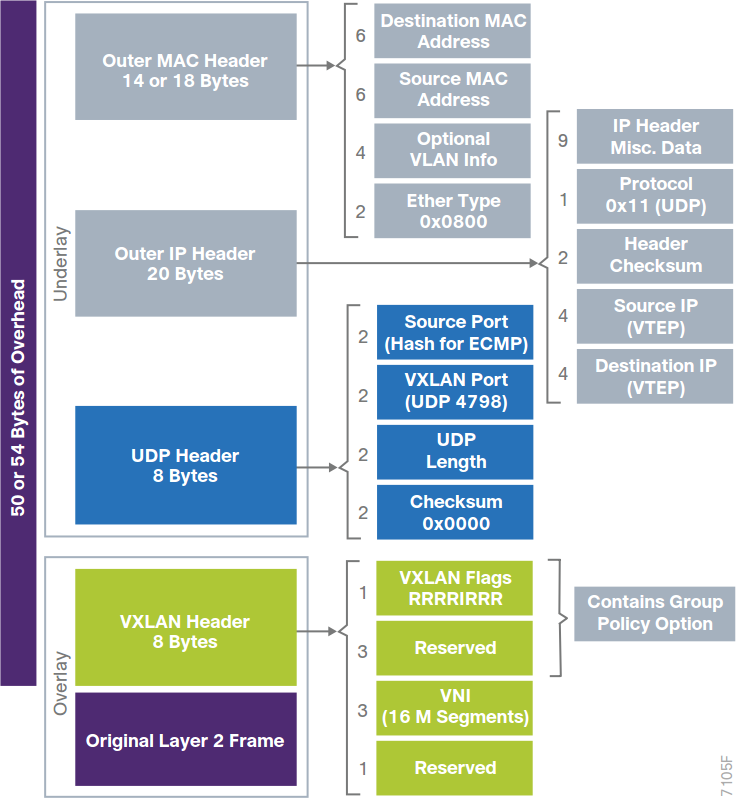
\includegraphics[width=0.7\linewidth]{img/RFC7348-VXLAN-Header.png}\\[1px]
	\caption{RFC7348 VXLAN Header}
	\label{fig:RFC7348 VXLAN Header}
\end{figure}

Das SDA Fabric verwendet die VXLAN Data Plane, um das vollständige ursprünglichen Layer 2 Frame bereitzustellen und verwendet zusätzlich LISP als Control Plane, um die Endpunkt zu VTEP Zuordnungen aufzulösen. Das SDA Fabric ersetzt 16 der reservierten Bits im VXLAN-Header, um bis zu 64'000 SGTs zu transportieren. Dabei wird ein modifiziertes VXLAN-GPO-Format verwendet.

Der VNI wird einer virtuellen Routing- und Weiterleitungsinstanz für Layer 3 Overlays zugeordnet, während ein Layer 2 VNI einer VLAN-Broadcastdomäne zugeordnet wird. Beide bieten den Mechanismus zur Isolierung von Data und Control Plane für jedes einzelne virtuelle Netzwerk. Die SGT trägt Gruppenmitgliedschaftsinformationen von Benutzern und stellt eine Data Plane Segmentierung innerhalb des virtualisierten Netzwerks bereit. \cite{sda-designguide}

\subsection{Slack}
Slack ist ein webbasierter Instant-Messaging-Dienst des US-amerikanischen Unternehmens Slack Technologies zur Kommunikation innerhalb von Arbeitsgruppen. Slack erlaubt, Nachrichten auszutauschen, mit Einzelpersonen oder in einer Gruppe zu chatten sowie gemeinsam Dokumente zu bearbeiten. Andere Online-Dienste wie Dropbox, Google Drive oder GitHub lassen sich in Slack integrieren.

\subsection{Infoblox}
Infoblox ist einer der führenden Hersteller für DNS-, DHCP-, TFTP und IP-Adress-Management Appliance (IPAM). Die Integration von Infoblox ermöglicht dem DNA Center die IPAM-Funktionen von Infoblox zu nutzen. Dafür werden beispielsweise die IP-Adresspools zwischen dem DNA Center und Infoblox synchronisiert. Mit dieser Integration können IP-Adresszuweisungen automatisiert werden, was eine richtlinienbasierte Bereitstellung in einer einzigen Operation ermöglicht und so die betriebliche Effizienz verbessert. \\
Infoblox ermöglicht die automatische Überprüfung der Netzwerkinfrastrukturen, die Konfiguration sowie Anpassung an die jeweiligen Compliance-Vorgaben. Mittels DNS-, DHCP-, TFTP und IP-Adress-Management Appliance (IPAM) werden wichtige Kontrollfunktionen für Endgeräte und Anwendungen bereitgestellt. Dank der DNS-Management-Software-Appliance kann stets der Überblick über Ihre IP-Adressbereiche behalten und die Verteilung der DNS- und DHCP-Daten überprüft und automatisiert werden. Reportings älterer sowie aktueller Daten können dank einer zuverlässigen Netzwerkdatenbank sowie Grid-Technologie erstellt werden.\cite{infoblox} \\

\begin{figure}[H]
	\centering
	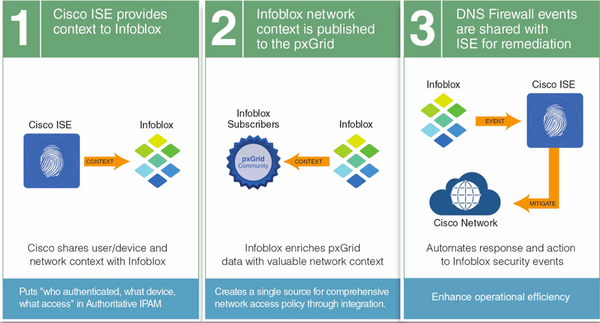
\includegraphics[width=0.7\linewidth]{img/infoblox-ise.png}\\[1px]
	\caption{Zusammenspiel Infoblox und ISE}
	\label{fig:Zusammenspiel Infoblox und ISE}
\end{figure}

Die gemeinsame Lösung von Infoblox ActiveTrust und Cisco Identity Services Engine (ISE) verbessert die Genauigkeit und Aktualität von Sicherheitsmaßnahmen, erhöht die Sichtbarkeit und erleichtert den Austausch von Informationen zwischen Netzwerk- und Sicherheitsteams. Cisco teilt den Gerätekontext mit Infoblox, während der Infoblox-Netzwerkkontext in pxGrid veröffentlicht wird, sodass Netzwerkadministratoren die Reaktionszeit für die Sicherheit automatisieren und verkürzen können.\cite{infoblox-communityblog}



\subsection{SDA Mechanismus Beispiel}

Ausgangslage: Wenn ein IP Paket über SD-A von PC1 172.16.1.1/24 nach PC2 10.0.2.34/24 geschickt wird, was passiert mit dem Paket?

\begin{figure}[H]
	\centering
	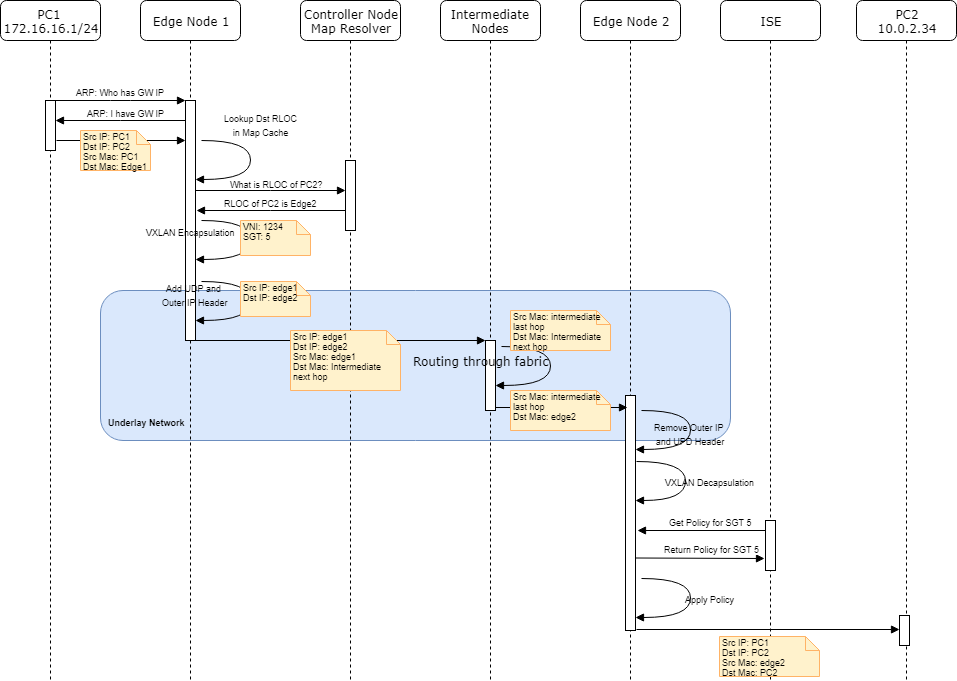
\includegraphics[width=16cm]{img/SDA_Mechanismus-NewVersion.png}
	\caption{SDA Mechanismus}
	\label{fig:SDA Mechanismus}
\end{figure}

Als erstes wird vom PC1 ein ARP Lookup an den Default GW gesendet. Dieser erhält eine Antwort vom Edge Node 1 (GW ist Anycast Adresse und wird von jedem Edge Node beantwortet). Nachfolgend sendet der PC1 sein Paket an den GW. Der Edge Node 1 führt ein RLOC Lookup im lokalen Map Cache aus. Falls kein Eintrag im lokalen Cache vorhanden ist, sendet er ein RLOC Lookup an den Map Resolver. Von diesem Map Resolver erhält der Edge Node 1 den RLOC von PC2 falls vorhanden. Ist dieser nicht bekannt, wird der Border Node verwendet. Nun erfolgt die VXLAN Encapsulation (SGT 5, VNI1234) und es wird der UDP und Outer IP Header hinzugefügt (Underlay Network). Das Paket wird nun an die RLOC IP (Destination Edge Node) weitergesendet. Sollten Intermediate Nodes vorhanden sein, wird das Paket durch diese geroutet, bis der Edge Node 2 das Paket erhält. Nun werden der UDP und Outer IP Header wieder entfernt (Underlay Netowork) und es geschieht die VXLAN Decapsulation. Nun wird die Policy für SGT 5 beim ISE angefragt. Dieser gibt die dazugehörigen Policies zurück und wendet diese auf das Paket an. Je nach Policy wird das Paket weitergesendet oder verworfen. In diesem Fall wird die Policy angewendet und an das Ziel, den PC2 weitergeleitet.



